% \subsection{Characterization of Performance}

Before embarking on a computational campaign that will consume 150M core
hours on the NCSA Blue Waters machine, we studied the scalability of HTBAC so
as to determine optimal workflow sizing and resource utilization for the
ESMACS protocol. The goal is twofold: (1) understanding the invariance of
HTBAC execution time over the number of workflow pipelines executed; and (2)
studying how the performance of EnTK and RP varies in relation to the size of
workflow.

% ---------------------------------------------------------------------------
\subsection{Experiment Design}\label{ssec:exp_design}

We designed two experiments to measure HTBAC, EnTK and RP weak scalability
when executing an increasing number of concurrent pipelines. According to the
use case described in Section~\ref{sec:htbac}, each pipeline consists of
seven stages, each stage with a single task. EnTK manages the queuing of the
tasks in accordance with the order and concurrency mandated by stages and
pipelines: For each pipeline, each stage is executed sequentially while
pipelines are executed concurrently.

Experiment 1 measures the baseline behavior of EnTK and RP with the workflow
of the ESMACS protocol and a null workload (\textmd{/bin/sleep 0}). The goal
is to isolate the overheads of EnTK and RP from the specifics of the
executables of the workflow and the overheads of the resources. The null
workload does not require data staging, I/O on both memory and disk, or
communication over network.

Experiment 2 replicates the design of Experiment 1 but it executes the
workflow of the ESMACS protocol with the actual simulation and data for the
EGFR kinase workload. The comparison between the two experiments enables
performance analysis of EnTK and RP to understand whether and how the size of
the executed workflow affects its overheads. Further, Experiment 2 shows also
whether HTBAC execution time is sensitive to the number of concurrent
pipelines executed.

Both experiments measure the weak scalability of HTBAC, EnTK and RP\@. This
means that the ratio between the number of pipelines and cores is kept
constant by design. While an investigation of strong scalability would
contribute to a better understanding of the behavior of HTBAC, EnTK and RP,
it is of limited interest for the current use case. The driving goal of HTBAC
is to increase throughput by a means of concurrency of pipelines, not in the
number of sequential executions per core. This is a driving motivation to
target large HPC machines instead of so-called HTC infrastructures.

% ---------------------------------------------------------------------------
\subsection{Experiment Setup}\label{ssec:exp_setup}

We perform both Experiment 1 and 2 on NCSA's Blue Waters---a 13.3 petaFLOPS
Cray, with 32 Interlago cores/50 GB RAM per node, Cray Gemini, Lustre shared
file system. Currently, we exclusively use CPUs on Blue Waters as GPUs are
not required by our use case. RCT support the use of both type of
architectures and we previously benchmarked the use of GPUs.

We perform our experiments from a virtual machine hosted in Europe. This
helps to simulate the conditions in which the experimental campaign will be
performed by the research group at UCL\@. This is relevant because, as most
HPC resources, Blue Waters does not allow for executing applications on the
login node of the cluster. To this end, RCTs support \textmd{gsissh} for X509
authentication and authorization.

Table~\ref{tab:exp} shows the setup for Experiment 1 and 2. The ESMACS
protocol is executed with up to 25 concurrent but independent pipelines and
therefore their concurrent execution does not entail communication overhead.
Further, the EGFR kinase studies can benefit from greater concurrency because
potential HTBAC users may wish to extend their protocols beyond the current
scale of ESMACS\@. Consistently, our experiments push the boundaries of
current scale by executing 8, 16, 32, 64 and 128 concurrent pipelines.

\begin{table*}[t]
\centering
\caption{Experiment 1 executes the 7 stages of the ESMACS protocol with
a null workload; Experiment 2 uses the actual MD workload of the ESMACS
protocol. ESMACS protocol with EGFR kinase workload: (1) Untar configuration
files; (2) Preprep; (3) Minimize with decreasing restraints; (4)
Equilibration: NVT simulation at 50K, with restraints; (5) Equilibration: NPT
simulation at 300K, with decreasing restraints; (6) Equilibration: NPT at
300k, no constraints; (7) Tarball output files.}\label{tab:exp}
\begin{tabular}{llllllll}
\toprule
\textbf{Experiment ID}      &
\textbf{Protocol}           &
\textbf{Workload}           &
\textbf{\# Trials}          &
\textbf{\# Pipelines}       &
\textbf{\# Stages}          &
\textbf{\# Tasks}           &
\textbf{\# Cores per pilot} \\
\toprule
%
1                           &
ESMACS                      &
Null workload               &
2                           &
8, 16, 32, 64, 128          &
7                           &
7                           &
64, 128, 256, 512, 1024     \\
%
2                           &
ESMACS                      &
EGFR kinase Workload        &
2                           &
8, 16, 32, 64, 128          &
7                           &
7                           &
64, 128, 256, 512, 1024     \\
\bottomrule
\end{tabular}
\end{table*}

EnTK uses RP to acquire resources via a single pilot. The size of the pilot is
contingent upon characterization of performance, in this case, weak
scalability. Accordingly, we request the maximum number of cores required by
the workload as the number of cores in a pilot. We use between 64 and 1024
cores in Experiment 2 as the NAMD executable used in stages 3, 4, 5, and 6
requires 8 cores. Stages 1, 2 and 7 require instead 1 core. The null workload
of Experiment 1 requires only 1 core per stage but we request the same number
of cores as for Experiment 2 to be able to compare the overheads of both EnTK
and RP across experiments.


All experiments use EnTK version 0.4.7 and RP version 0.42. The MD engine used
is NAMD-MPI\@. The equilibration tasks of stage 4 and 6 are assigned 5000
timesteps while the task of stage 5 requires 55000 timesteps. We ran two
trials of both the null and MD workload at each pipeline configurations.

% ---------------------------------------------------------------------------
\subsection{Results}\label{ssec:exp_results}

First we characterize the overhead of EnTK and RP in the null workload, where
we isolate the overhead introduced by the two systems
(Figure~\ref{fig:exp1}). We see a (slightly) superliner increase of EnTK
overhead, between 0.1 and 1.8 seconds. This overhead depends on the number of
tasks that need to be translated in-memory from a Python object to a compute
unit (CU) description. As such, it is expected to grow proportionally to the
number of tasks, barring some competition of resources.

\begin{figure}
  \centering
  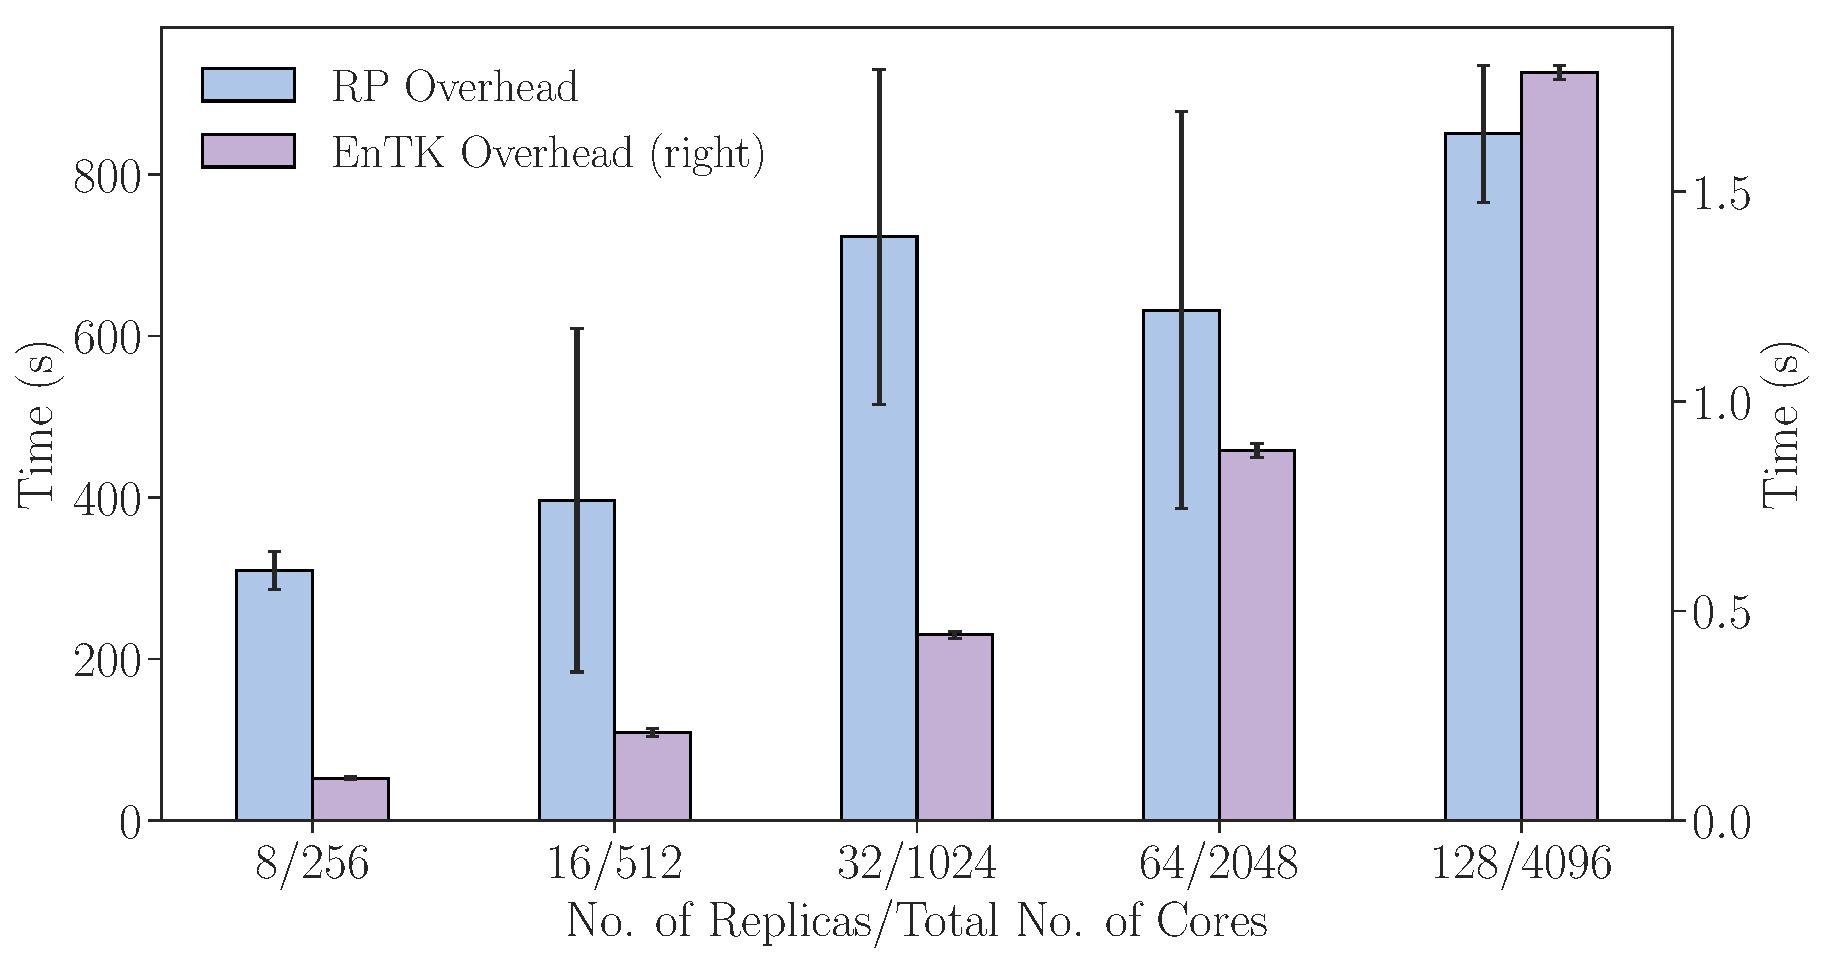
\includegraphics[width=\columnwidth]{null_workload_overheads.pdf}
  \caption{Overheads of Ensemble Toolkit (EnTK) and RADICAL-Pilot (RP) when
           executing HTBAC using a null workload. We plot the baseline
           EnTK/RP overheads without the application workload across two
           trials per pipeline configuration.}\label{fig:exp1}
\end{figure}

RP overhead is also, on average, superlinear but with a much greater
variance. This variance is due to mainly two factors: Network latency and
filesystem latency on the HPC resource. EnTK submits CU descriptions to the
MongoDB used by RP, and the RP pilot pulls these descriptions from the same
database. As described in Section~\ref{ssec:exp_setup}, this pull operation
occurs over a wide area network, introducing varying amounts of latency.
Further, RP writes and reads the CU descriptions multiple times to and
from the shared filesystem of the HPC machine. Together, these two factors
introduce delays in the scheduling of the CUs.

When the workload includes the EGFR kinase, we see (Figure~\ref{fig:exp2}) that the
RP overhead becomes on average less than 10\% of the average total execution
time (TTX), defined as \(TTX = TTC - T_q\) where \(TTC\) is
time-to-completion and \(T_q\) is time spent queuing on the HPC machine. We further break down TTX into the time-to-completion per stage, where stages 1,2, and 7 perform file movements, while stages 3,4,5, and 6 execute NAMD tasks. At this level we notice that the time-to-completion of the NAMD stages are essentially invariant across pipelines of different size while file movement stages exhibit linearly increasing behavior. In addition, when accounting for variance, RP overheads also show linear weak scaling behavior. 
%We also notice the TTX is essentially invariant across pipelines of different size
%and that, when accounting for variance, RP overheads also shows linear weak
%scaling behavior. 
As expected, EnTK overhead remains superlinear and
comparable to the one measured in Experiment 1. This is because in both
experiments EnTK overhead depends on the number of tasks translated to CU
descriptions.

\begin{figure}
  \centering
  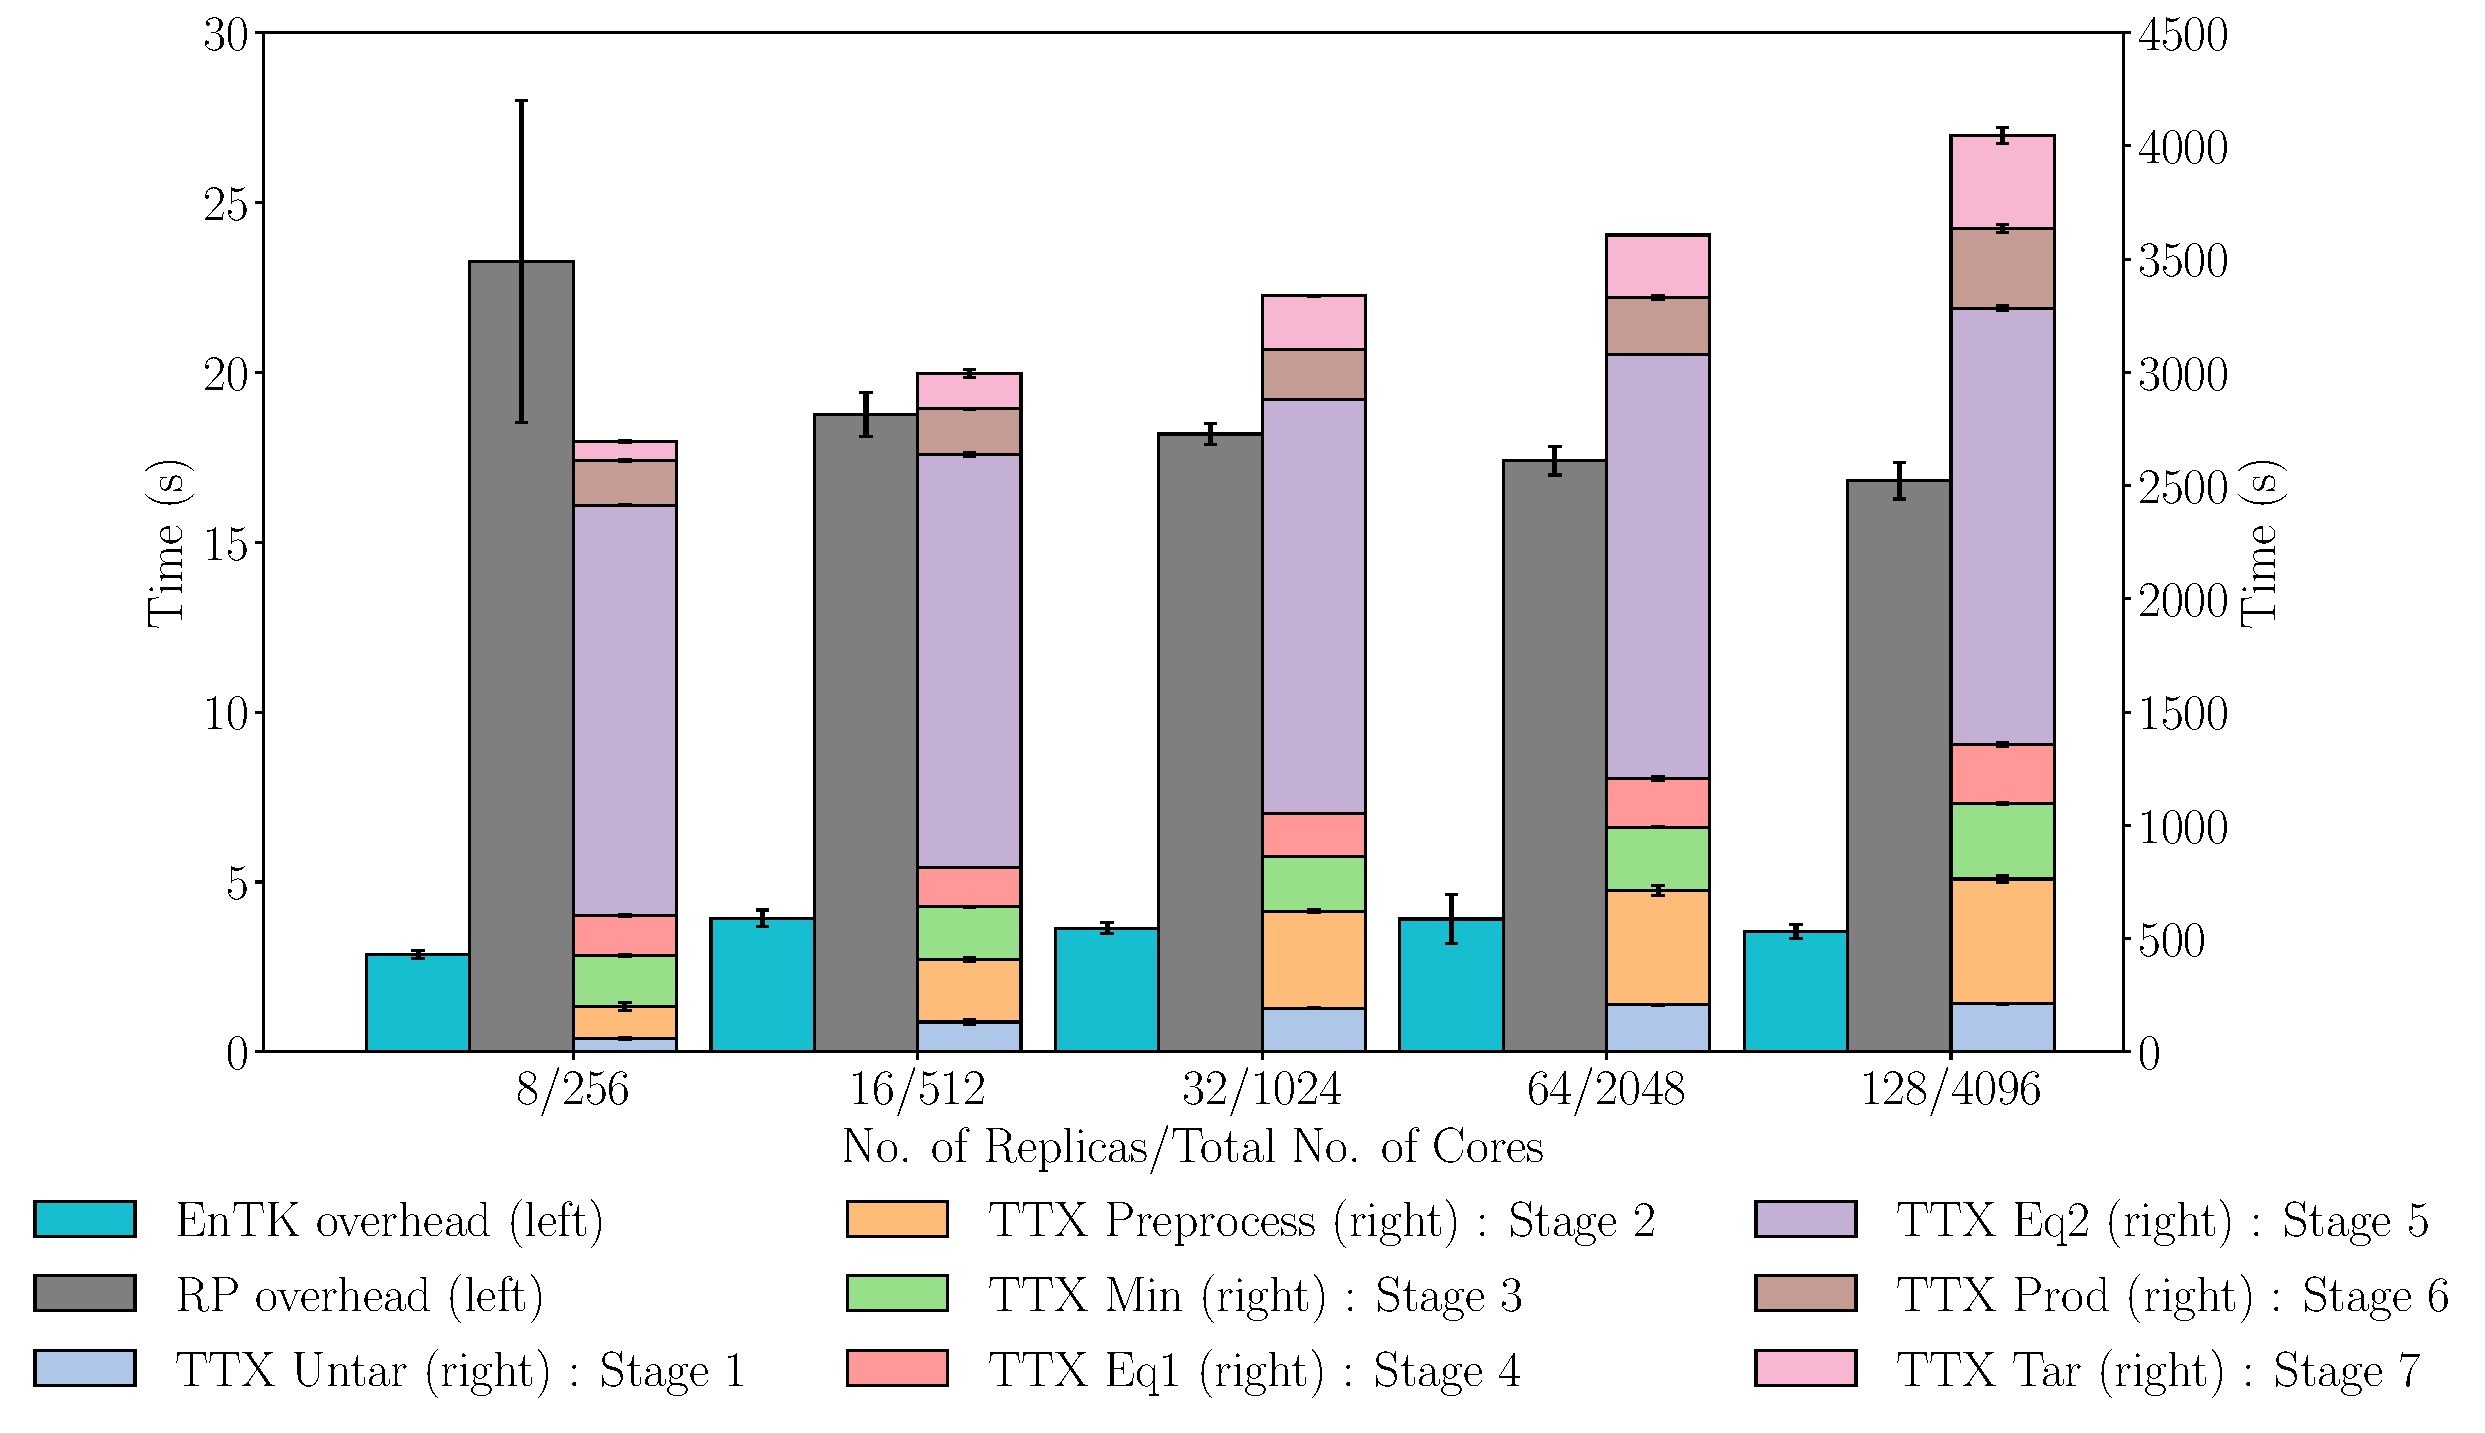
\includegraphics[width=\columnwidth]{esmacs_32.pdf}
  \caption{Introducing the use-case EGFR kinase workload, we observe
  similar EnTK/RP overhead behavior as with the null workload with higher
  values as the number of pipelines increases. We show a breakdown of TTX of 
  each stage (Stage 1 - Stage 7). Across pipeline configurations, TTX and RP overheads 
  (accounting for the error bars) show
  weak scaling performance.}\label{fig:exp2}
\end{figure}

Experiments 1 and 2 show how the overheads of both EnTK and RP tend to be
invariant across type of workload executed. Their scaling behavior and, to
some approximation, their absolute values are comparable between
Figure~\ref{fig:exp1} and~\ref{fig:exp2}. This is relevant because it shows
that the systems used to coordinate and execute the ESMACS protocol add a
constant and comparatively not relevant overhead to the execution of NAMD\@.
